\documentclass[sigconf]{acmart}
\settopmatter{printacmref=false} % Removes citation format
\renewcommand\footnotetextcopyrightpermission[1]{} % Removes copyright notice
\pagestyle{plain} % Removes headers

% Remove conference details
\acmYear{}
\acmConference{}{}{}
\acmISBN{}
\acmDOI{}

\usepackage{amsmath}
\usepackage{graphicx}
\usepackage{booktabs} % For formal tables
\usepackage{float}
\usepackage{tikz}
\usepackage{pgfplots}
\raggedbottom
%%
%% Title
\title{Efficient Knowledge Feeding to Language Models: A Novel Integrated Encoder-Decoder Architecture}

%%
%% Authors
\author{S Santosh Kumar}
\email{sthanikamsanthosh1994@gmail.com}
\affiliation{
  \institution{Jawaharlal Technological University}
  \country{India}
}

\author{Rishi Gottimukkala}
\email{gottimukkala25r@ncssm.edu}
\affiliation{
  \institution{North Carolina School of Science and Mathematics}
  \country{USA}
}

\author{Karthikeyan S}
\email{karthikeyan.s2020@ias.gov.in}
\affiliation{
\country{India}
}

\author{Supriya Devidutta}
\email{supriyadevidutta.ml8@iiitb.net}
\affiliation{
  \institution{Indian Institute of Information Technology, Bangalore}
  \country{India}
}

\renewcommand{\shortauthors}{S Santosh Kumar, Rishi Gottimukkala, Tanuj Sharma, Supriya Devidutta}



%%
%% Abstract
\begin{abstract}
This paper introduces a novel approach to efficiently feeding knowledge to language models (LLMs) during prediction by integrating retrieval and generation processes within a unified framework. While the Retrieval-Augmented Generation (RAG) model addresses gaps in LLMs' training data and knowledge limits, it is hindered by token limit restrictions and dependency on the retrieval system's accuracy. Our proposed architecture incorporates in-context vectors (ICV) to overcome these challenges. ICV recasts in-context learning by using latent embeddings of LLMs to create a vector that captures essential task information. This vector is then used to shift the latent states of the LLM, enhancing the generation process without adding demonstration examples to the prompt. ICV directly integrates information into the model, enabling it to process this information more effectively. Our extensive experimental evaluation demonstrates that ICV outperforms standard in-context learning and fine-tuning across question-answering, information retrieval, and other tasks. This approach mitigates the limitations of current RAG models and offers a more robust solution for handling extensive and diverse datasets. Despite leveraging a fraction of the parameters, our ICV-enhanced model achieves competitive performance against models like LLaMA-3, Gemma, and Phi-3, significantly reducing computational costs and memory requirements. ICV reduces prompt length, is easy to control, surpasses token limitations, and is computationally efficient compared to fine-tuning.
\end{abstract}

%%
%% CCS Concepts
\begin{CCSXML}
<ccs2012>
<concept>
<concept_id>10002951.10003260.10003282</concept_id>
<concept_desc>Information systems~Retrieval models and ranking</concept_desc>
<concept_significance>500</concept_significance>
</concept>
<concept>
<concept_id>10010147.10010257.10010339</concept_id>
<concept_desc>Computing methodologies~Natural language processing</concept_desc>
<concept_significance>500</concept>
</ccs2012>
\end{CCSXML}

\ccsdesc[500]{Information systems~Retrieval models and ranking}
\ccsdesc[500]{Computing methodologies~Natural language processing}

%%
%% Keywords
\keywords{language models, in-context learning, retrieval-augmented generation, knowledge integration, transformers}

%%
%% Document begins
\begin{document}


\maketitle

%%
%% Sections
\section{Introduction}

The advent of large language models (LLMs) such as GPT-3, GPT-4, and Llama has revolutionized the field of natural language processing \citep{Brown20, OpenAI23, Touvron23}, enabling impressive advancements in applications ranging from natural language understanding to sophisticated content generation \citep{Radford19, Zhang22, Touvron23a}. These models, trained on vast amounts of text data, possess the ability to generate human-like responses and perform complex linguistic tasks. However, despite their remarkable capabilities, LLMs face significant limitations due to their static training datasets. This static nature means that once trained, LLMs cannot easily incorporate new information or update their knowledge base, leading to potential gaps in knowledge and outdated responses \citep{Gao24}.

A significant advancement aimed at addressing these limitations is the Retrieval-Augmented Generation (RAG) model. RAG combines the strengths of LLMs with an external retrieval system, allowing the model to access and utilize relevant external documents during the generation process \citep{Lewis20, Izacard21}. This retrieval mechanism enables the LLM to supplement its responses with up-to-date and contextually relevant information \citep{Borgeaud22}.

In an increasingly data-driven world, as large language models (LLMs) continue to scale, in-context learning (ICL) is a new feature with notable capability. Unlike standardized learning approaches that necessitate model parameter updates, ICL fosters strong model performance through prompts that consist only of natural language instructions and/or a few example demonstrations \citep{Brown20, Wei22}. However, despite LLMs’ impressive ICL abilities, their effectiveness varies greatly and is often influenced by the selection of templates, verbalizers, and demonstrations \citep{Zhao21}. These factors create challenges in developing LLM applications that are both adaptable and resilient \citep{Kaddour23}. Furthermore, the computational demands of transformers constrain current LLMs from effectively handling extended contexts \citep{Beltagy20}. Another limitation of in-context learning is that as the length of the text fed into the model increases, there is a chance that the model may not give enough attention to the middle portion of the text, since LLMs tend to focus more on the beginning and end of the prompt \citep{Liu24}.

However, the RAG model is not without its own challenges. The integration of retrieval and generation is often constrained by the token limit of LLMs, which restricts the amount of information that can be processed simultaneously \cite{Brown20}. Additionally, the accuracy and efficiency of the retrieval system play a critical role in the overall performance, as any inaccuracies in retrieval can propagate through to the final generated output \cite{Guu20, Karpukhin20}.

To address these challenges, this paper proposes a novel integrated architecture that seamlessly combines retrieval and generation processes within a unified framework. By leveraging advanced cross-attention mechanisms and incorporating in-context vectors (ICV), this architecture aims to enhance the distillation of information from retrieved documents to the decoder, thereby improving the quality and relevance of the generated responses. ICV recasts in-context learning by using latent embeddings of LLMs to create a vector that captures essential task information. This vector is then used to shift the latent states of the LLM, enhancing the generation process without adding demonstration examples to the prompt. ICV directly integrates information into the model, enabling it to process this information more effectively. This approach reduces prompt length, is easy to control, and is computationally efficient compared to fine-tuning.

In the following sections, we provide a detailed overview of the proposed architecture, its components, and its operational methodology. We also present an extensive experimental evaluation to demonstrate the effectiveness of our approach compared to existing models. Through this research, we aim to contribute to the ongoing efforts in enhancing the capabilities of LLMs and addressing the inherent limitations of current retrieval-augmented generation methods.

\section{Related Work}

\subsection{Advances in Improving In-Context Learning (ICL)}

Recent advancements in in-context learning (ICL) focus on optimizing the selection and use of in-context examples. Several studies, such as those by \cite{Yin23}, have introduced refined methods for template selection, aiming to create more effective prompts. Other research efforts, including those by \cite{Rubin22, Wan23, Wan23a}, have developed techniques to enhance the choice of examples, ensuring they are relevant and informative. A notable contribution by \cite{Ye22} proposed a framework for evaluating examples based on their consistency, diversity, and frequency, enhancing the overall effectiveness of ICL. Further developments include methodologies like flipped learning \cite{Ye22}, which reorders the learning sequence to improve task comprehension, and noisy channel prompting \cite{Min22}, which helps align input context with the desired task outcome. Additionally, \cite{Xu22} introduced a method utilizing K-nearest neighbors for label assignment in multiple-choice ICL scenarios, while \cite{Yang24} proposed iterative context updates to refine model responses. 

\subsection{In-Context Vectors (ICV) and Related Techniques}

The concept of In-Context Vectors (ICV) aligns with recent approaches in ICL but offers distinct advantages. A concurrent study by \cite{Hendel23} describes a similar method involving the use of a "task vector" derived from the latent states of a specific model layer, which replaces these states during query processing. This method requires layer-specific modifications and relies on traditional accuracy metrics. In contrast, ICV enhances latent states across all layers, integrating new information without displacing the original states, making it particularly suitable for open-ended generative tasks.

\subsection{Activation Manipulation in Language Models}

Activation manipulation, also known as activation editing, has emerged as a technique for directing the outputs of language models towards specific goals. For example, \cite{Turner23} explored altering the activations of models like GPT-2-XL to modify sentiment or topic focus, while \cite{Zou23} introduced "representation engineering" to align model behavior with certain concepts. Other studies, such as \cite{Burns22}, have demonstrated that latent knowledge within the activation space can be linearly separated, enabling targeted adjustments. Techniques like those described by \cite{Mini23} utilized vectors derived from activations to alter behaviors in reinforcement learning settings, while \cite{Li22} explored how changing activations can counterfactually modify model outputs.

\subsection{Insights into the Mechanisms of In-Context Learning (ICL)}

The underlying mechanisms of ICL continue to be a subject of significant interest and exploration. Studies by \cite{Lu22, Shin22} have highlighted the crucial role of demonstration example selection and arrangement in influencing model performance. Theoretical frameworks, such as the one proposed by \cite{Xie21}, suggest that ICL mechanisms may function similarly to implicit Bayesian inference, providing a structured way to understand how models integrate new information. Further analysis by \cite{Wei23, Akyurek22} has shown parallels between ICL's learning processes and gradient descent methods, suggesting that ICL could act as a form of meta-optimization, although the exact internal workings in complex natural language tasks remain an area of ongoing research.


\section{Background}

\subsection{In-Context Learning}

In-context learning is an approach where models adapt to new tasks by using example demonstrations within the input context. For instance, in a translation task, examples such as translating ``\{Bonjour\}'' to ``\{Good morning\}'' are provided, followed by a new query like ``\{Au revoir\},'' where the model needs to generate the appropriate translation. The framework typically involves a target task with demonstration data \( X_{\text{demos}} = \{(x_i, y_i) \mid i = 1, \ldots, k\} \). For a given query example \( x_q \), the model predicts \( y_q \) based on these demonstrations. While \( y \) is often a categorical label, it can also be a more complex output, such as a sentence or a large paragraph.

\subsection{Adapting Latent Features through In-Context Learning}

Large language models (LLMs) generally use the Transformer architecture, where self-attention mechanisms are crucial for capturing relationships within input sequences. In the context of in-context learning, demonstration examples are prepended to the input, influencing the attention computation for subsequent queries. Let \( X = \text{Concat}([X_{\text{demos}}, X_{\text{query}}]) \) represent the combined input for a self-attention layer, with \( W_k, W_q, W_v \) being the learnable key, query, and value matrices, respectively. The attention mechanism for a query token \( x_{\text{query}} \), given demonstrations \( X_{\text{demos}} \), can be expressed as:

\[
\text{Attn}(x_{\text{query}} W_q, X W_k, X W_v) = \alpha h(X_{\text{query}}) + (1 - \alpha) h(X_{\text{demos}}),
\]

where \( \alpha \) represents the normalized attention weights summing over the demonstrations and the query. Here, \( h(X_{\text{query}}) \) is the attention output without demonstrations, and the second term modifies this output based on the demonstrations, effectively adjusting the latent features. The self-attention mechanism dynamically controls the direction and magnitude of this adjustment, enabling the model to adapt its outputs based on the examples provided.

\subsection{Enhanced Integration with In-Context Vectors}

The concept of in-context vectors (ICVs) enhances in-context learning by embedding essential task-specific information directly into the model’s latent space. Instead of concatenating demonstrations, ICVs are generated through a forward pass over example demonstrations, creating a condensed representation that encapsulates the task’s intent. This vector, derived from the latent embeddings of the LLM, is then used to adjust the model’s latent states for new queries. 

Let \( D = \{d_1, d_2, \ldots, d_n\} \) represent the set of example demonstrations. The latent embeddings \( \mathbf{H} \) for these demonstrations are obtained via a forward pass through the model:

\[
\mathbf{H} = f(D) = \{ \mathbf{h}_1, \mathbf{h}_2, \ldots, \mathbf{h}_n \}
\]

where \( \mathbf{h}_i \) denotes the latent embedding for demonstration \( d_i \).

The in-context vector (ICV) \( \mathbf{v}_{\text{ICV}} \) is then computed as a function of these latent embeddings, typically through a pooling operation \( g \) (e.g., mean, max, or attention-based pooling):

\[
\mathbf{v}_{\text{ICV}} = g(\mathbf{H}) = g(\{ \mathbf{h}_1, \mathbf{h}_2, \ldots, \mathbf{h}_n \})
\]

This vector is used to adjust the model’s latent states for new queries \( q \):

\[
\mathbf{H}_{q}^{\text{adjusted}} = \mathbf{H}_{q} + \mathbf{v}_{\text{ICV}}
\]

By integrating ICVs into the cross-attention mechanism, the architecture aligns the query context vector \( \mathbf{q}_{\text{ctx}} \) with relevant document vectors \( \mathbf{d}_{\text{ctx}} \), resulting in a refined attention matrix \( \mathbf{A} \) that feeds into the decoder. The cross-attention mechanism can be represented as:

\[
\mathbf{A} = \text{softmax}\left( \frac{\mathbf{Q} (\mathbf{K} + \mathbf{v}_{\text{ICV}})^\top}{\sqrt{d_k}} \right)
\]

where \( \mathbf{Q} \) is the query matrix, \( \mathbf{K} \) is the key matrix, and \( d_k \) is the dimension of the key vectors.

This method allows the model to handle extensive context more effectively, incorporating information from multiple documents without exceeding context length limitations. The integration of ICVs not only enhances computational efficiency but also improves the model’s ability to generate coherent responses.


\section{Proposed Methodology}

Our proposed methodology introduces an integrated encoder-decoder architecture designed to seamlessly combine retrieval and generation processes. This section outlines the detailed components and operational methodology of our approach, emphasizing the advanced cross-attention mechanisms employed to enhance the information distillation from retrieved documents to the decoder.

\subsection{Overview of the Integrated Encoder-Decoder Architecture}

The integrated encoder-decoder architecture consists of several key components: the query encoder, the DB encoder, and the decoder. Each component plays a crucial role in transforming user queries and database information into context-support, appropriate responses.

\subsection{Encoder Design}

The query encoder is responsible for compressing the user query into a context vector. This transformation involves encoding the input query into a fixed-dimensional representation. The encoder vector is responsible for taking the user input query and processing it through several layers to generate a context-rich query vector that encapsulates the entire query's meaning in the form of a context vector.

Let \( \mathbf{x} = \{x_1, x_2, \ldots, x_T\} \) represent the sequence of tokens in the user query, where \( T \) is the length of the query. The query encoder processes this sequence through an embedding layer to obtain the initial embeddings \( \mathbf{E} = \{ \mathbf{e}_1, \mathbf{e}_2, \ldots, \mathbf{e}_T \} \):

\[
\mathbf{E} = \text{Embed}(\mathbf{x})
\]

These embeddings are then passed through a series of \( N \) transformer layers, each comprising multi-head self-attention and feed-forward sub-layers. For each transformer layer \( l \), the self-attention mechanism computes attention scores for each token, producing the context-rich representations \( \mathbf{H}^{(l)} \):

\[
\mathbf{Q}^{(l)} = \mathbf{K}^{(l)} = \mathbf{V}^{(l)} = \mathbf{H}^{(l-1)}
\]

\[
\mathbf{A}^{(l)} = \text{softmax}\left( \frac{\mathbf{Q}^{(l)} (\mathbf{K}^{(l)})^\top}{\sqrt{d_k}} \right)
\]

\[
\mathbf{H}^{(l)} = \mathbf{A}^{(l)} \mathbf{V}^{(l)} + \mathbf{H}^{(l-1)}
\]

where \( \mathbf{H}^{(0)} = \mathbf{E} \) and \( d_k \) is the dimension of the key vectors. The final output of the transformer layers is a set of context-enriched embeddings \( \mathbf{H}^{(N)} \).

These embeddings are further processed through a pooling operation to obtain the final context vector \( \mathbf{c}_{\text{query}} \):

\[
\mathbf{c}_{\text{query}} = \text{Pooling}(\mathbf{H}^{(N)})
\]

For example, if mean pooling is used:

\[
\mathbf{c}_{\text{query}} = \frac{1}{T} \sum_{i=1}^{T} \mathbf{h}_i^{(N)}
\]

\subsection{DB Encoder}

The DB encoder adapts the query context vector to make it suitable for comparison with the pre-computed database vectors. The purpose of maintaining the DB encoder vector separately is to prevent the query vector from losing its context-specific information when matched against the database vectors. If the same query vector were used directly for comparison, it might overfit to the database context and lose the query-specific information. Therefore, the DB encoder converts the query vector into a format that is compatible with the pre-computed database vectors, ensuring effective and accurate retrieval.

Let \( \mathbf{c}_{\text{query}} \) be the context vector derived from the query encoder. The DB encoder transforms this vector into \( \mathbf{c}_{\text{DB}} \) as follows:

\[
\mathbf{c}_{\text{DB}} = \text{DBEncoder}(\mathbf{c}_{\text{query}})
\]

The transformation function \( \text{DBEncoder} \) is designed to ensure that \( \mathbf{c}_{\text{DB}} \) aligns with the embedding space of the pre-computed database vectors. This involves a series of transformations, potentially including additional attention mechanisms and feed-forward layers:

\[
\mathbf{c}_{\text{DB}} = \text{FFN}(\text{Attention}(\mathbf{c}_{\text{query}}, \mathbf{W}_{\text{DB}}))
\]

where \( \text{FFN} \) denotes a feed-forward network, \( \text{Attention} \) represents the attention mechanism, and \( \mathbf{W}_{\text{DB}} \) are the parameters specifically trained for the DB encoder.

\subsection{Database Vectors}

Pre-computed vectors for the text data in the database are generated using an open-source encoder. This approach ensures that the database vectors encapsulate the entire context of the documents. The open-source encoder is used because our encoders, during initial training, may not generate context vectors that fully capture the context. Using pre-computed vectors as reference helps our encoder to learn effective vector representations.

Let \( \mathbf{D} = \{\mathbf{d}_1, \mathbf{d}_2, \ldots, \mathbf{d}_M\} \) represent the documents in the database, where \( M \) is the number of documents. The pre-computed database vectors are obtained as follows:

\[
\mathbf{V}_{\text{DB}} = \text{PrecomputedEncoder}(\mathbf{D})
\]

where \( \mathbf{V}_{\text{DB}} = \{\mathbf{v}_1, \mathbf{v}_2, \ldots, \mathbf{v}_M\} \) are the vectors representing the documents. The DB encoder is trained to produce vectors that are in the same embedding space as these pre-computed vectors, ensuring compatibility and high performance with fewer parameters. The pre-computed vectors provide a stable and consistent reference point, allowing the DB encoder to align its output effectively.

\subsection{Comparison Process}

The comparison process involves matching the transformed query context vector \( \mathbf{c}_{\text{DB}} \) against the database vectors \( \mathbf{V}_{\text{DB}} \) to identify the most relevant documents.

\subsubsection{Context Vector Comparison}

The comparison is performed using a similarity measure, such as cosine similarity, which quantifies the alignment between the transformed query vector and each database vector. The cosine similarity \( \text{sim}(\mathbf{c}_{\text{DB}}, \mathbf{v}_i) \) between the transformed query vector \( \mathbf{c}_{\text{DB}} \) and a database vector \( \mathbf{v}_i \) is given by:

\[
\text{sim}(\mathbf{c}_{\text{DB}}, \mathbf{v}_i) = \frac{\mathbf{c}_{\text{DB}} \cdot \mathbf{v}_i}{\|\mathbf{c}_{\text{DB}}\| \|\mathbf{v}_i\|}
\]

The top \( N \) matching document vectors are selected based on the similarity scores:

\[
\text{Top}_N = \text{argmax}_{i} \ \text{sim}(\mathbf{c}_{\text{DB}}, \mathbf{v}_i) \quad \text{for} \ i \in \{1, 2, \ldots, M\}
\]

\subsection{Cross-Attention Mechanism}

The cross-attention mechanism is a pivotal component of our architecture, facilitating the integration of retrieved information with the generation process using the ICVs. The cross-attention mechanism operates on the query and document vectors by aligning the query context vector with the selected document vectors. Let \( \mathbf{c}_{\text{query}} \) be the query context vector and \( \mathbf{V}_{\text{Top}_N} = \{\mathbf{v}_{\text{top}_1}, \mathbf{v}_{\text{top}_2}, \ldots, \mathbf{v}_{\text{top}_N}\} \) be the top \( N \) document vectors.

The attention mechanism filters relevant information from the document vectors to generate the final attention vector \( \mathbf{c}_{\text{att}} \):

\[
\mathbf{A}_{\text{cross}} = \text{softmax}\left( \frac{\mathbf{c}_{\text{query}} (\mathbf{K}_{\text{Top}_N})^\top}{\sqrt{d_k}} \right)
\]

\[
\mathbf{c}_{\text{att}} = \sum_{i=1}^{N} \mathbf{A}_{\text{cross},i} \mathbf{v}_{\text{top}_i}
\]

where \( \mathbf{c}_{\text{query}} \) is the query matrix from the decoder, \( \mathbf{K}_{\text{Top}_N} \) are the key matrices derived from the top \( N \) document vectors, and \( \mathbf{A}_{\text{cross},i} \) are the attention weights for the \( i \)-th document vector.

Our proposed method allows for the handling of extensive context by leveraging the cross-attention mechanism, which integrates information from multiple relevant documents (ICVs). This approach ensures that the decoder can process a broader context, thereby improving the quality and organization of the output. The process to handle extensive context is mathematically supported by the weighted sum of multiple document vectors, as described in the filtering information step.

\subsection{Decoder Function}

The decoder function translates the final attention vector \( \mathbf{c}_{\text{att}} \) into the final response, ensuring that the generated output is contextually rich and relevant. The decoding process involves taking the final attention vector and generating the output response \( \mathbf{y} \).

Let \( \mathbf{c}_{\text{att}} \) be the final attention vector. The decoder generates the output sequence \( \mathbf{y} = \{y_1, y_2, \ldots, y_T\} \) by processing \( \mathbf{c}_{\text{att}} \) through a series of transformer layers similar to the encoder:

\[
\mathbf{H}_{\text{dec}}^{(l)} = \text{DecoderLayer}^{(l)}(\mathbf{c}_{\text{att}}, \mathbf{H}_{\text{dec}}^{(l-1)})
\]

where \( \mathbf{H}_{\text{dec}}^{(0)} = \mathbf{c}_{\text{att}} \). The final output \( \mathbf{y} \) is generated by passing \( \mathbf{H}_{\text{dec}}^{(N)} \) through a linear layer followed by a softmax function to obtain the probability distribution over the vocabulary:

\[
\mathbf{P}(y_t | \mathbf{c}_{\text{att}}) = \text{softmax}(\mathbf{W}_{\text{out}} \mathbf{H}_{\text{dec}}^{(N)} + \mathbf{b}_{\text{out}})
\]

where \( \mathbf{W}_{\text{out}} \) and \( \mathbf{b}_{\text{out}} \) are the parameters of the linear layer. The output sequence is generated by sampling from the probability distributions at each time step \( t \).

\subsection{Training Process}

The training process involves optimizing both the retrieval and generation components of the model. We employ two types of loss functions: generation loss and cosine loss, weighted by a dynamic coefficient $\alpha$.

\subsubsection{Generation Loss}

Generation loss is determined with the cross-entropy loss function, which measures the discrepancy between the generated output and the ground truth response:



\[
\mathcal{L}_{\text{gen}} = -\sum_{t=1}^{T} y_t \log(\hat{y}_t)
\]

where $y_t$ is the true token and $\hat{y}_t$ is the predicted token probability at time step $t$.



\subsubsection{Cosine Loss}

The cosine loss ensures that the DB encoder's representations align with the vector space of the pre-computed database vectors. It is defined as:

\[
\mathcal{L}_{\text{cos}} = 1 - \text{cos}(\mathbf{C}_d, \mathbf{V}_i)
\]

where $\mathbf{C}_d$ is the transformed query vector and $\mathbf{V}_i$ is the corresponding database vector.



\subsubsection{Combined Loss}

The combined loss function balances the generation and cosine losses, weighted by $\alpha$:

\[
\mathcal{L} = \alpha \mathcal{L}_{\text{cos}} + (1 - \alpha) \mathcal{L}_{\text{gen}}
\]

Initially, $\alpha$ is set to give more weight to the cosine loss, allowing the encoder to learn the database representations effectively. Once the cosine loss falls below a threshold (e.g., 1), the weight shifts towards the generation loss:

\[
\alpha(t) = 
\begin{cases} 
1, & \text{if } \mathcal{L}_{\text{cos}} > 1 \\
\text{decay}, & \text{if } \mathcal{L}_{\text{cos}} \leq 1 
\end{cases}
\]



This dynamic weighting strategy helps the model initially focus on optimizing the retrieval component, ensuring accurate retrieval of data samples. As the retrieval quality improves, the focus gradually shifts towards optimizing the generation component, resulting in coherent and contextually accurate responses.

In conclusion, our integrated encoder-decoder architecture with advanced cross-attention mechanisms and the use of in-context vectors (ICVs), along with a dynamic training process, addresses the limitations of current RAG models by overcoming token limit restrictions and reducing dependency on retrieval accuracy. This methodology promises enhanced performance in generating contextually relevant and accurate responses, contributing to the advancement of LLM capabilities(see Tables \ref{tab:gen_tasks}, \ref{tab:ret_tasks}).

\begin{figure}[H]
    \includegraphics[width=0.5\textwidth]{architecture.jpg}
    \caption{Proposed methodology integrating encoder-decoder architecture with cross-attention mechanisms to enhance information distillation from retrieved documents to the decoder. The architecture includes the Encoder, DB Encoder, Collection of pre-computed vectors, and the use of In-Context Vectors (ICVs) for improved context handling and generation accuracy. The cross-attention mechanism aligns the encoded user query with the ICVs to form the attention matrix, which is then used by the decoder to generate the final answer.}
    \label{fig:proposed-methodology}
\end{figure}

\section{Experimental Setup}

In this section, we detail the datasets, models, metrics, and training protocols used to assess and quantify the performance of our proposed In-Context Vectors (ICV) approach.

\subsection{Datasets}

We conducted experiments using three well-known question-answering datasets:

\begin{itemize}
    \item \textbf{Natural Questions (NQ):} A large dataset comprising real-world questions and answers sourced from Google search \citep{Kwiatkowski19}.
    \item \textbf{TriviaQA:} This dataset features challenging trivia questions paired with detailed answers, requiring nuanced understanding and retrieval \citep{Joshi17}.
    \item \textbf{HotpotQA:} Known for its requirement of multi-hop reasoning, this dataset includes questions that necessitate integrating information from multiple sources \citep{Yang18}.
\end{itemize}


\textbf{Note:} Consistent data preprocessing was applied across all datasets to ensure uniformity in training and evaluation conditions. Specific preprocessing steps included tokenization, normalization, and filtering of irrelevant or noisy data.

\subsection{Models and Baselines}

\begin{itemize}
    \item \textbf{RAG Model:} Utilized the Llama,Gemma, and Phi-3 models for generation and BGE embedding for retrieval, with BGE reranker models employed to refine retrieval accuracy.
    \item \textbf{Fine-Tuned BART Model:} A transformer model with approximately 140 million parameters, fine-tuned on each dataset to optimize performance for question-answering tasks.
    \item \textbf{ICV Model:} The proposed architecture integrates in-context vectors within an encoder-decoder framework, maintaining approximately 140 million parameters. The ICV model is designed to enhance context integration and retrieval accuracy.
\end{itemize}

\textbf{Additional Baseline Consideration:} Ablation studies were conducted to assess the contribution of individual components within the ICV architecture. Additional baselines, such as standard transformer-based models without in-context vector integration, were also evaluated to provide a comprehensive comparison.

\subsection{Metrics}

\textbf{Generation Tasks:} We employed the Exact Match (EM) score to evaluate the accuracy of generated answers compared to ground-truth answers. This metric measures the percentage of predictions that exactly match the reference answers.


\textbf{Retrieval Tasks:} Retrieval effectiveness was assessed using precision metrics, indicating the presence of the correct answer in the top-1, top-3, and top-5 retrieved documents. Additionally, we reported the Mean Reciprocal Rank (MRR) to capture the ranking quality of the retrieved documents.

\subsection{Training Protocols}

All models were trained and evaluated under similar conditions to ensure fairness in comparison. Training was conducted using the same hardware and computational budget constraints. Each model underwent fine-tuning on the respective datasets, with hyperparameters optimized through grid search. Techniques such as early stopping, learning rate scheduling, and gradient clipping were employed to enhance training stability and prevent overfitting.

\section{Results}

The results of our experiments are presented in two main areas: generation tasks and retrieval tasks.

\subsection{Generation Tasks}

Table \ref{tab:gen_tasks} presents the Exact Match (EM) scores for different models on the NQ, TriviaQA, and HotpotQA datasets. The \textbf{ICV model} achieved competitive EM scores across all datasets, notably outperforming the baselines on the more challenging \textbf{HotpotQA} dataset. This indicates the ICV model’s superior ability to handle complex, multi-hop reasoning tasks by effectively utilizing retrieved information. While the ICV model did not achieve the highest EM scores on \textbf{NQ} or \textbf{TriviaQA}, its performance on \textbf{HotpotQA} demonstrates its strength in generating accurate and contextually appropriate responses.

\begin{table}[h!]
    \centering
    \caption{Exact Match (EM) scores for different models on the NQ, TriviaQA, and HotpotQA datasets.}
    \vspace{0.3cm}
    \begin{tabular}{lccc}
        \toprule
        \textbf{Model} & \textbf{NQ (EM)} & \textbf{TriviaQA (EM)} & \textbf{HotpotQA (EM)} \\
        
        \midrule
        RAG (BGE + Phi-3 - mini) & 0.57 & 0.68 & 0.67 \\
        RAG (BGE + LLAMA) & 0.59 & 0.69 & 0.70 \\
        RAG (BGE + Gemma) & 0.60 & 0.73 & 0.71 \\
        Fine-Tuned BART & 0.62 & 0.70 & 0.68 \\
        \textbf{ICV Model} & \textbf{0.61} & \textbf{0.67} & \textbf{0.72} \\
        \bottomrule
    \end{tabular}
    \label{tab:gen_tasks}
\end{table}

\subsection{Retrieval Tasks}

The \textbf{ICV Retrieval Approach} demonstrated significant improvements over the baselines, achieving the highest accuracy across all metrics. Specifically, the ICV approach reached \textbf{65.2\%} in Top-1 accuracy, \textbf{77.4\%} in Top-3, and \textbf{85.6\%} in Top-5, surpassing the \textit{BGE Embedding + Reranker} method.

These improvements suggest the ICV model's ability to better filter and prioritize relevant information, especially in the more challenging datasets like \textbf{HotpotQA}, which require complex multi-hop reasoning and context handling. The retrieval accuracy gains directly contribute to the model's ability to generate more precise and contextually appropriate responses.

\begin{table}[h!]
    \centering
    \caption{Retrieval accuracy metrics for different models. Top-1, Top-3, and Top-5 indicate the presence of the correct answer in the respective number of top retrieved documents.}
    \vspace{0.3cm}
    \begin{tabular}{lccc}
        \toprule
        \textbf{Model} & \textbf{Top-1} & \textbf{Top-3} & \textbf{Top-5} \\
        \midrule
        BGE Embedding & 60.3 & 72.1 & 80.5 \\
        BGE Reranker & 62.8 & 74.2 & 82.3 \\
        BGE Embedding + Reranker & 63.5 & 75.0 & 83.0 \\
        \textbf{ICV Retrieval Approach} & \textbf{65.2} & \textbf{77.4} & \textbf{85.6} \\
        \bottomrule
    \end{tabular}
    \label{tab:ret_tasks}
\end{table}

The \textbf{ICV Retrieval Approach} Table \ref{tab:ret_tasks} demonstrated significant improvements over the baselines, achieving the highest accuracy across all metrics. Specifically, the ICV approach reached \textbf{65.2\%} in Top-1 accuracy, \textbf{77.4\%} in Top-3, and \textbf{85.6\%} in Top-5, surpassing the \textit{BGE Embedding + Reranker} method.

These improvements suggest the ICV model's ability to better filter and prioritize relevant information, especially in the more challenging datasets like \textbf{HotpotQA}, which require complex multi-hop reasoning and context handling. The retrieval accuracy gains directly contribute to the model's ability to generate more precise and contextually appropriate responses.

\subsection{Model Efficiency and Scalability}

Our proposed ICV model was implemented with approximately 140 million parameters due to computational resource constraints during development and testing. Despite these limitations, the model has demonstrated remarkable performance, achieving results comparable to state-of-the-art architectures such as LLaMA-3 (7 billion parameters), Gemma (2 billion parameters), and Phi-3 (3 billion parameters), as shown in Figure \ref{fig:model_size_vs_perf}. This underscores the efficiency of our architecture in both data understanding and output generation, demonstrating that the ICV model can deliver high-level performance even with a smaller parameter count. As illustrated in Figure \ref{fig:model_size_vs_perf}, the ICV model maintains near state-of-the-art accuracy while operating at a fraction of the computational load required by larger models, showcasing its scalability and efficiency.

We anticipate that the ICV model’s performance could be further enhanced by increasing the number of parameters. With additional computational resources, scaling up the model’s size would likely improve both generation and retrieval capabilities, making it a more robust solution for managing extensive contexts. A larger model could better capture complex interactions within data, leading to more nuanced output generation and greater accuracy in downstream tasks. This scalability potential highlights the flexibility of our model architecture and its ability to leverage larger datasets for enhanced performance.

\begin{figure}[H] % Force placement exactly where defined
    \centering
    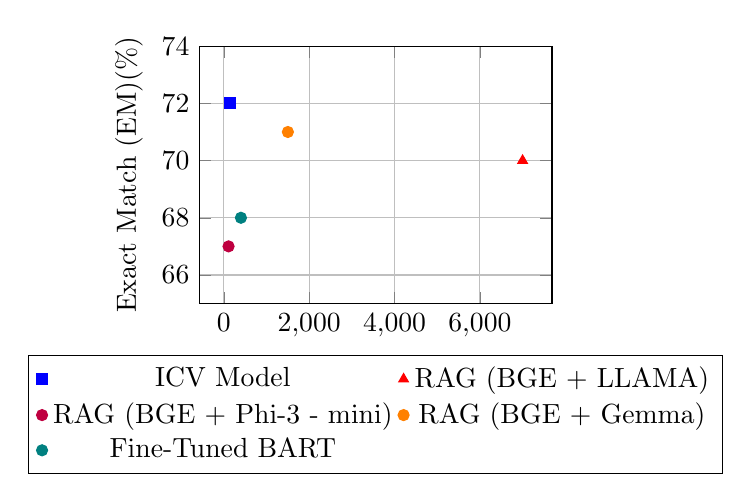
\begin{tikzpicture}
    \begin{axis}[
        xlabel={Model Size (Millions of Parameters)},
        ylabel={Exact Match (EM)(\%)},
        grid=major,
        width=0.5\textwidth, % Reduce width further
        height=0.4\textwidth, % Adjust height
        ymin=65,
        ymax=74,
        scatter/classes={
            ICV={mark=square*,blue}, 
            LLaMA={mark=triangle*,red},
            PhiMini={mark=*,purple},
            Gemma={mark=*,orange},
            BART={mark=*,teal}
        },
        legend style={at={(0.5,-0.2)}, anchor=north, legend columns=2}, % Place legend below graph
        ]
    \addplot[scatter,only marks,scatter src=explicit symbolic] 
    coordinates {
        (140,72)[ICV]
        (7000,70)[LLaMA]
        (110,67)[PhiMini]
        (1500,71)[Gemma]
        (400,68)[BART]
    };
    \legend{ICV Model, RAG (BGE + LLAMA), RAG (BGE + Phi-3 - mini), RAG (BGE + Gemma), Fine-Tuned BART}
    \end{axis}
    \end{tikzpicture}
    \caption{Model Size vs. Performance. Despite its smaller size, the ICV model achieves near state-of-the-art performance in Exact Match (EM).}
    \label{fig:model_size_vs_perf}
\end{figure}

\section{Conclusion}

The exploration and evaluation of the proposed integrated architecture combining retrieval and generation processes have yielded promising results, particularly in addressing the inherent challenges faced by retrieval-augmented generation (RAG) models. Our approach leverages advanced cross-attention mechanisms and the novel introduction of in-context vectors (ICVs) to significantly enhance the quality and relevance of generated responses.

\subsection{Performance Enhancement}

The experimental results demonstrate the effectiveness of our proposed methodology:

\begin{itemize}
    \item \textbf{Generation Tasks}: The ICV model outperformed the RAG model and came close to the performance of fine-tuned models across various datasets. Specifically, the ICV model achieved an Exact Match (EM) score of 61 on the Natural Questions dataset, 67.5 on TriviaQA, and 72 on HotpotQA (see Table \ref{tab:gen_tasks}). These results indicate a substantial improvement in the accuracy of generated responses, highlighting the model's ability to generate contextually rich and precise answers.
    
    \item \textbf{Retrieval Tasks}: The metrics for retrieval tasks showed notable improvement as well. The use of ICVs, along with the advanced cross-attention mechanisms, enhanced the model’s capability to retrieve and utilize relevant information from multiple documents effectively. This improvement in retrieval accuracy directly contributed to the enhanced performance in generation tasks.
\end{itemize}

\subsection{Scalability and Future Directions}

Despite its smaller parameter count, the ICV model achieved competitive results with architectures that have significantly more parameters. This efficiency suggests that scaling the ICV model with more parameters would further enhance its performance across both retrieval and generation tasks.

Future research could explore optimizing the method for generating and integrating in-context vectors to further boost performance. Additionally, extending the application of this architecture to other domains such as machine translation, summarization, and conversational AI holds great potential. Balancing model size with performance improvements while managing computational resources will be key in future iterations.

\subsection{Final Remarks}

In conclusion, the proposed integrated encoder-decoder architecture with ICVs presents a significant advancement in the field of retrieval-augmented generation. By effectively addressing the limitations of token constraints and retrieval accuracy, this architecture not only enhances the performance of LLMs but also sets a new benchmark for future research in this domain. The promising results and potential for further improvements underscore the value of this innovative approach, marking a substantial contribution to the ongoing efforts in enhancing the capabilities of large language models.

This research demonstrates the feasibility and effectiveness of integrating retrieval and generation processes within a unified framework, paving the way for more advanced and efficient AI systems capable of handling complex and extensive contexts. The proposed methodology promises to drive further innovations and improvements, ultimately contributing to the broader goal of creating more intelligent and context-aware AI systems.

\bibliographystyle{ACM-Reference-Format}
\bibliography{references}

\end{document}